\chapter{One-Locus Models of Selection}
\begin{quotation}
"Socrates consisted of the genes his parents gave him, the experiences they and his environment later provided, and the growth a development mediated by numerous meals. For all I know, he may have been very successful in the evolutionary sense of leaving numerous offspring. His phenotype, nevertheless, was utterly destroyed by the hemlock and has never since been duplicated. The same argument holds also for genotypes. With Socrates' death, not only did his phenotype disappear, but also his genotype.[…] The loss of Socrates’ genotype is not assuaged by any consideration of how prolifically he may have reproduced. Socrates' genes may be with us yet, but not his genotype, because meiosis and recombination destroy genotypes as surely as death."
\end{quotation}

\paragraph{Fitness}

As we have seen, natural selection occurs when there are differences between individuals in fitness. We may define fitness in various ways. Most commonly, it is defined with respect to the contribution of a phenotype or genotype to the next generation. 
Differences in fitness can arise at any point during the life cycle. For instance, different genotypes or phenotypes may have different survival probabilities from one stage in their life to the stage of reproduction (viability), or they may differ in the number of offspring produced (fertility), or both. Here, we define the absolute fitness of a genotype as the expected number of offspring of an individual of that genotype. Differences in fitness among genotypes drive allele frequency change.\\


\subsection{Haploid selection model}
We start out by modeling selection in a haploid model, as this is mathematically relatively simple.


Let the number of individuals carrying alleles $A_1$ and $A_2$ in generation $t$ be $P_t$ and $Q_t$. Then, the relative frequencies at time $t$ of alleles $A_1$ and $A_2$ are $p_t = P_t / (P_t + Q_t)$ and $q_t = Q_t / (P_t + Q_t) = 1 - p_t$. Further, assume that individuals of type $A_1$ and $A_2$ on average produce $W_1$ and $W_2$ offspring individuals, respectively. We call $W_i$ the absolute fitness.\\

Therefore, in the next generation, the absolute number of carriers of $A_1$ and $A_2$ are $P_{t+1} = W_1 P_t$ and $Q_{t+1} = W_2 Q_t$, respectively. The mean absolute fitness of the population at time $t$ is
\begin{equation}
	\label{eq:meanAbsFit}
	\Wbar_t = W_1 \frac{P_t}{P_t + Q_t} + W_2 \frac{Q_t}{P_t + Q_t} = W_1 p_t + W_2 q_t,	
\end{equation}
i.e.\ the sum of the fitness of the two types weighted by their
relative frequencies. Note that the mean fitness depends on time, as
it is a function of the allele frequencies, which are themselves time
dependent. \\

The frequency of allele $A_1$ in the next generation is then given by
\begin{equation}
	\label{eq:eq:recHaplMod1}
	p_{t+1} = \frac{P_{t+1}}{P_{t+1} + Q_{t+1}} = \frac{W_1 P_t}{W_1 P_t + W_2 Q_t}
	%= \frac{W_1 (P_t + Q_t)p_t}{W_1 (P_t + Q_t)p_t + W_2 (P_t + Q_t)q_t}
	= \frac{W_1 p_t}{W_1 p_t + W_2 q_t} = \frac{W_1}{\Wbar_t} p_t.
\end{equation}


Importantly, eqn.\ (\ref{eq:eq:recHaplMod1}) tells us that the change in $p$ only depends on a ratio of fitnesses. Therefore, we need to specify fitness only up to an arbitrary constant. As long as we multiply all fitnesses by the same value, that constant will cancel out and eqn.\ (\ref{eq:eq:recHaplMod1}) will hold. Based on this argument, it is very common to scale absolute fitnesses by the absolute fitness of one of the genotypes, e.g.\ the most or the least fit genotype, to obtain relative fitnesses. Here, we will use $w_i$ for the relative fitness of genotype $i$. If we choose to scale by the absolute fitness of genotype $A_1$, we obtain the relative fitnesses $w_1 = W_1/W_1 = 1$ and $w_2 = W_2/W_1$.\\
Without loss of generality, we can therefore rewrite eqn.\ (\ref{eq:eq:recHaplMod1}) as
\begin{equation}
	\label{eq:recHaplMod2}
	p_{t+1} = \frac{w_1}{\wbar} p_t,
\end{equation}
dropping the dependence of the mean fitness on time in our notation, but remembering it.
The change in frequency from one generation to the next is then given by
\begin{equation}
\Delta p_t = p_{t+1} - p_t= \frac{ w_1 p_t}{ \wbar} - p_t = \frac{w_1 p_t - \wbar p_t}{\wbar} = \frac{w_1 p_t - (w_1 p_t + w_2 q_t) p_t}{\wbar} = \frac{w_1 - w_2}{\wbar} p_t q_t,
\label{eq:deltap_haploid}
\end{equation}
recalling that $q_t = 1 - p_t$.\\

Assuming that the fitnesses of the two alleles are constant over time,
the number of the two allelic types $\tau$ generations after time $t$ are
$P_{t+\tau} = (W_1)^{\tau} P_t$ and $Q_{t+\tau}=  (W_2)^{\tau} Q_t$, respectively. Therefore, the relative frequency of allele $A_1$ after $\tau$ generations past $t$ is
\begin{equation}
	p_{t+\tau} = \frac{ (W_1)^{\tau} P_t}{ (W_1)^{\tau} P_t+(W_2)^{\tau} Q_t} = \frac{ (w_1)^{\tau} P_t}{ (w_1)^{\tau} P_t+(w_2)^{\tau} Q_t} = \frac{p_t}{p_t + (w_2/w_1)^{\tau} q_t},
	\label{eq:haploid_tau_gen}
\end{equation}
where the last step includes dividing the whole term by $(w_1)^{\tau}$ and switching from absolute to relative allele frequencies.\\

Rearranging eqn.\ \eqref{eq:haploid_tau_gen} and setting $t = 0$, we can work out the time $\tau$ for the frequency of $A_1$ to change from $p_0$ to $p_{\tau}$. First, we write
\begin{equation}
	p_{\tau} = \frac{p_0}{p_0 + (w_2/w_1)^{\tau} q_0}
\end{equation}
and rearrange this to obtain
\begin{equation}
	\label{eq:estTau}
	\frac{p_{\tau}}{q_{\tau}} = \frac{p_0}{q_0} \left(\frac{w_1}{w_2}\right)^{\tau}.
\end{equation}
Solving this for $\tau$ yields
\begin{equation}
	\label{eq:solTau}
	\tau = \log \left(\frac{p_{\tau} q_0}{q_{\tau} p_0}\right) /  \log\left(  \frac{w_1}{w_2} \right).
\end{equation}
\\

In practice, it is often helpful to parametrize the relative fitnesses $w_i$ in a specific way. For example, we may set $w_1 = 1$ and $w_2 = 1 - s$, where $s$ is called the selection coefficient. Using this parametrization, $s$ is simply the difference in relative fitnesses between the two alleles. Equation \eqref{eq:haploid_tau_gen} becomes
\begin{equation}
	\label{eq:haploid_tau_gen_expl}
	p_{t+\tau} = \frac{p_{t}}{p_{t} + q_{t} (1 - s)^{\tau}},
\end{equation}
as $w_2 / w_1 = 1 - s$. Then, if $s \ll 1$, we can approximate $(1-s)^{\tau}$ in the denominator by $\exp(-s\tau)$ to obtain
\begin{equation} \label{eq:haploid_logistic growth}
	p_{t+\tau} \approx \frac{p_t}{p_t + q_t e^{-s\tau}}.
\end{equation}
This equation takes the form of a logistic function. That is because
we are looking at the relative frequencies of two `populations' (of
alleles $A_1$ and $A_2$) that are growing (or declining)
exponentially, under the constraint that $p$ and $q$ always sum to 1. \\

Moreover, eqn.\ \eqref{eq:estTau} for the time $\tau$ it takes for a certain change in frequency to occur becomes
\begin{equation}
	\label{eq:estTauExpl}
	\tau = - \log \left(\frac{p_{\tau} q_0}{q_{\tau} p_0}\right) /  \log\left(1-s\right).
\end{equation}
Assuming again that $s \ll 1$, this simplifies to
\begin{equation}
	\label{eq:estTauExplSimpl}
	\tau \approx \frac{1}{s} \log \left(\frac{p_{\tau} q_0}{q_{\tau} p_0}\right).
\end{equation}


One particular case of interest is the time it takes to go from an absolute
frequency of 1 to near fixation in a population of size $N$.  In this case, we
have $p_0 = 1/N$, and we may set $p_{\tau} = 1 - 1/N$, which is very close to
fixation. Then, plugging these values into eqn.\ \eqref{eq:estTauExplSimpl}, we
obtain

\begin{align}
  tau &= \frac{1}{s} \log\left( \frac{1 - \nicefrac{2}{N} +
      \nicefrac{1}{N^2}}{\nicefrac{1}{N^2}} \right) \nonumber \\
  &\approx \frac{1}{s} (\log(N) + \log(N-2)) \nonumber \\
  &\approx \frac{2}{s} \log(N)  \label{eq:fixTimeSimpl}
\end{align}
%
where we make the approximations $N^2 - 2N + 1 \approx N^2 - 2N$ and later
$N-2 \approx N$.

\begin{tcolorbox}
\begin{question}
You are studying the frequency of antibiotic-resistant bacteria in a
patient.  Before administering the antibiotic the frequency of the 
resistance allele is $\nicefrac{1}{1000}$. You adminster the antibiotic,
alarming just 8 days later you find the frequency of the 
resistance allele to be $99\%$. Assume a generation time of $\nicefrac{1}{4}$ a day for
these bacteria. \\
What is the selection coefficient associated with the resistance to antibiotics?
\end{question}
\end{tcolorbox}
\paragraph{Haploid model with fluctuating selection}
We can now consider the case where the fitnesses depend on time \citep{Dempster:55}, and
say that $w_{1,t}$ and $w_{2,t}$ are the fitnesses of the two types in
generation $t$. The frequency of allele $A_1$ in generation $t+1$ is
\begin{equation}
p_{t+1} = \frac{w_{1,t}}{\wbar_t} p_t,
\end{equation}
which simply follows from eqn.\ \eqref{eq:recHaplMod2}.
The ratio of the frequency of allele $A_1$ to that of allele $A_2$ in generation $t+1$ is
\begin{equation}
\frac{p_{t+1}}{q_{t+1}} = \frac{w_{1,t}}{w_{2,t}}  \frac{p_{t}}{q_{t}}.
\end{equation}
Therefore, if we think of the two alleles starting in generation $t$ at
frequencies $p_t$ and $q_t$, then $\tau$ generations later,
\begin{equation}
\frac{p_{t+\tau}}{q_{t+\tau}} = \left(\prod_{i=t}^{\tau-1} \frac{w_{1,i}}{w_{2,i}}  \right) \frac{p_{t}}{q_{t}}.
\end{equation}
\\

The question of which allele is increasing or decreasing in frequency comes down
to whether $\left(\prod_{i=t}^{\tau-1} \nicefrac{w_{1,i}}{w_{2,i}}  \right)$ is
$>1$ or $<1$. As it is a little hard to think about this ratio, we can
instead take the $\tau^{\mathrm{th}}$ root of it and consider
\begin{equation}
\sqrt[\tau]{\left(\prod_{i=t}^{\tau-1} \frac{w_{1,i}}{w_{2,i}}  \right)} = \frac{\sqrt[\tau]{\prod_{i=t}^{\tau-1}w_{1,i}}}{\sqrt[\tau]{\prod_{i=t}^{\tau-1}w_{2,i}}}.
\end{equation}
The term $\sqrt[\tau]{\prod_{i=t}^{\tau-1}w_{1,i}}$ is the geometric mean fitness of allele
 $A_1$ over the $\tau$ generations past generation $t$. Therefore, allele $A_1$ will only increase
in frequency if it has a higher geometric mean fitness than allele $A_2$
(at least in our simple deterministic model). \\


\subsection{Diploid model}
We will now move on to a diploid model of a single locus with two segregating alleles.


\begin{figure}
\begin{center}
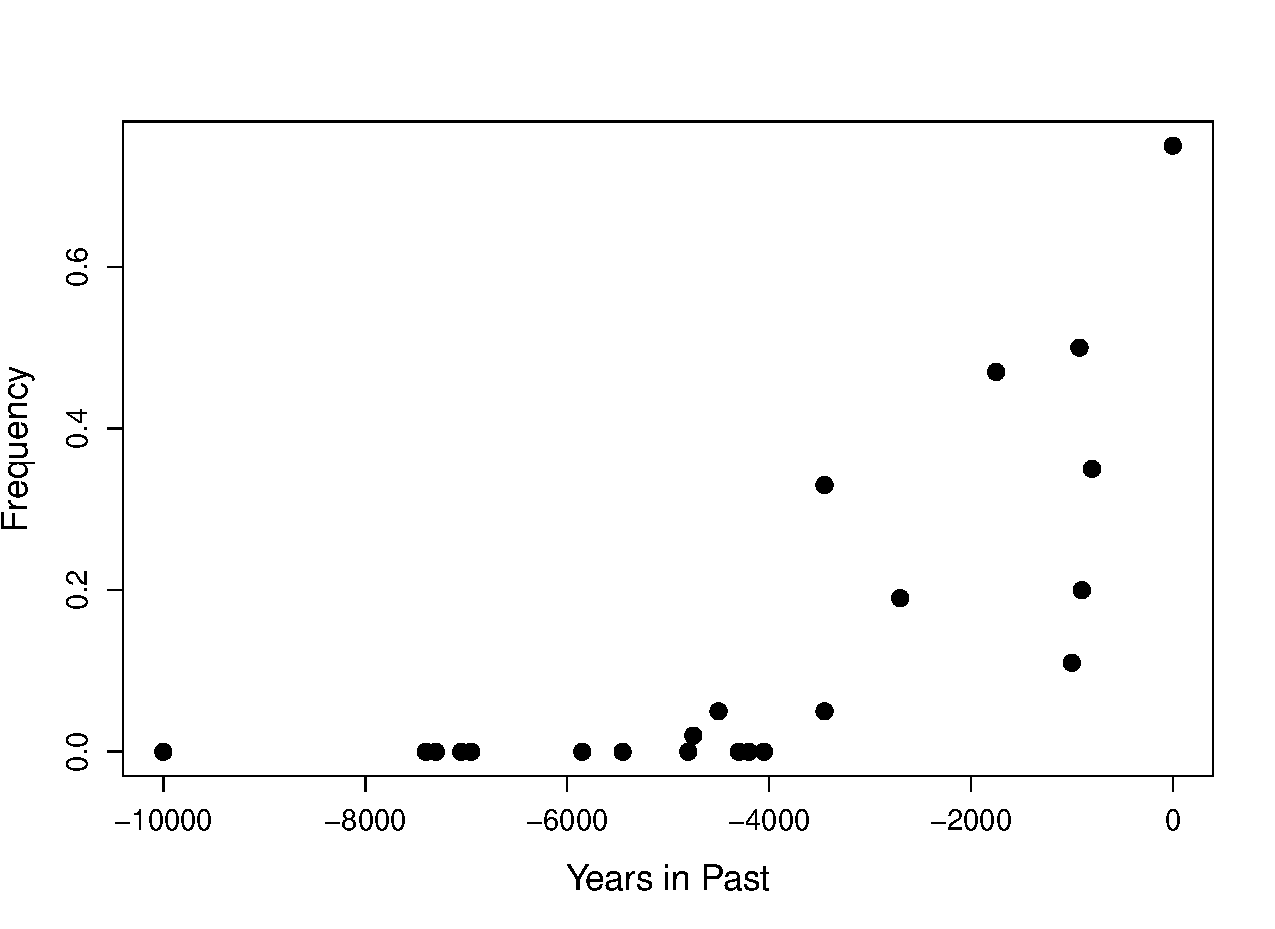
\includegraphics[width= \textwidth]{Rcode/Lactase_example/Lactase_freq_time.pdf}
\end{center}
\caption{} \label{fig:LCT_freqs}
\end{figure}



We will assume that the difference in fitness between the three
genotypes comes from differences in viability, i.e.\ differential
survival of individuals from the formation of zygotes to reproduction.  
We denote the absolute fitnesses of genotypes $A_1A_1$, $A_1A_2$, and $A_2A_2$ by $W_{11}$, $W_{12}$, and $W_{22}$. Specifically, $W_{ij}$ is the probability that a zygote of genotype $A_iA_j$ survives to reproduction.
Assuming that individuals mate at random, the number of zygotes that are of the three genotypes and form generation $t$ are
\begin{equation}
Np_t^2, ~~~  N2p_tq_t, ~~~ Nq_t^2.
\end{equation}

The mean fitness of the population of zygotes is then
\begin{equation}
	\Wbar_t = W_{11} p_t^2+W_{12} 2p_tq_t  +  W_{22} q_t^2.
\end{equation}
Again, this is simply the weighted mean of the genotypic fitnesses.
\\

How many zygotes of each of the three genotypes survive to reproduce?
An individual of genotype $A_1A_1$ has a probability of $W_{11}$ of
surviving to reproduce, and similarly for other genotypes. Therefore, the expected number of $A_1A_1$, $A_1A_2$, and $A_2A_2$ individuals who survive to reproduce is
\begin{equation}
	NW_{11} p_t^2, ~~~ NW_{12} 2p_tq_t , ~~~ N W_{22} q_t^2.
\end{equation}
It then follows that the total number of individuals who survive to
reproduce is
\begin{equation}
	N \left(W_{11} p_t^2+W_{12} 2p_tq_t  +  W_{22} q_t^2 \right).
\end{equation}
This is simply the mean fitness of the population multiplied by the
population size (i.e.\ $N \wbar$).\\

The relative frequency of $A_1A_1$ individuals at reproduction
is simply the number of $A_1A_1$ genotype individuals at reproduction ($NW_{11} p_t^2$)
divided by the total number of individuals who survive to reproduce
($N \Wbar$), and likewise for the other two genotypes.
Therefore, the relative frequency of individuals with the three different genotypes at reproduction is
\begin{equation}
	\frac{NW_{11} p_t^2}{N\Wbar}, ~~~ \frac{NW_{12} 2p_tq_t}{N\Wbar} , ~~~ \frac{N W_{22} q_t^2}{N\Wbar}
\end{equation}
(see Table \ref{dip_fitness_table}).\\

\begin{table*}
\begin{center}
\begin{tabular}{lccc}
\hline
& $A_1A_1$ & $A_1A_2$ & $A_2A_2$\\
\hline
Absolute no. at birth & $Np_t^2$ & $N2p_tq_t$ & $Nq_t^2$\\
Fitnesses & $W_{11}$ & $W_{12}$& $W_{22}$\\
Absolute no.\ at reproduction & $NW_{11} p_t^2$ & $NW_{12} 2p_tq_t$& $N W_{22} q_t^2$\\
Relative freq.\ at reproduction & $\frac{NW_{11} p_t^2}{N \Wbar} = \frac{W_{11}}{\Wbar} p_{t}^2$ & $\frac{NW_{12} 2p_tq_t}{N
\Wbar} = \frac{W_{12}}{\Wbar} 2 p_{t} q_{t}$ & $\frac{N W_{22} q_t^2}{N\Wbar} = \frac{W_{22}}{\Wbar} q_{t}^2$\\
\end{tabular}
\end{center}
\caption{Relative genotype frequencies after one episode of viability selection.} \label{dip_fitness_table}
\end{table*}

%\gc{Dobzhansky}

%\begin{center}
%\begin{tabular}{lccc}
%\hline
% & ST/ST & ST/CH & CH/CH \\  ##From Evolution encylopedia
%Eggs & 41 & 82 &27\\
%Adults & 25 & 74 & 12\\
%\end{tabular}
%\end{center}

As there is no difference in the fecundity of the three genotypes, the
allele frequencies in the zygotes forming the next generation are simply the
allele frequency among the reproducing individuals of the previous generation. Hence, the frequency of $A_1$ in generation $t+1$ is
\begin{equation}
	p_{t+1} = \frac{W_{11} p_t^2 + W_{12} p_tq_t}{\Wbar}
	\label{pgen_dip}.
\end{equation}
Note that, again, the absolute value of the fitnesses is irrelevant to
the frequency of the allele. Therefore, we can just as easily replace
the absolute fitnesses with the relative fitnesses. That is, we may replace $W_{ij}$ by $w_{ij} = W_{ij}/W_{11}$, for instance. \\

Each of our genotype frequencies is responding to selection in a
manner that depends just on its fitness compared to the mean fitness
of the population. For example the frequency of the $11$ homozygotes
increases from birth to adulthood in proportion to $W_{11}/Wbar$. In
fact we can estimate this fitness ratio for each genotype by comparing
the frequency at birth compared to adults. As an example of this we'll
look at some data from sticklebacks. 
\begin{marginfigure}
\begin{center}
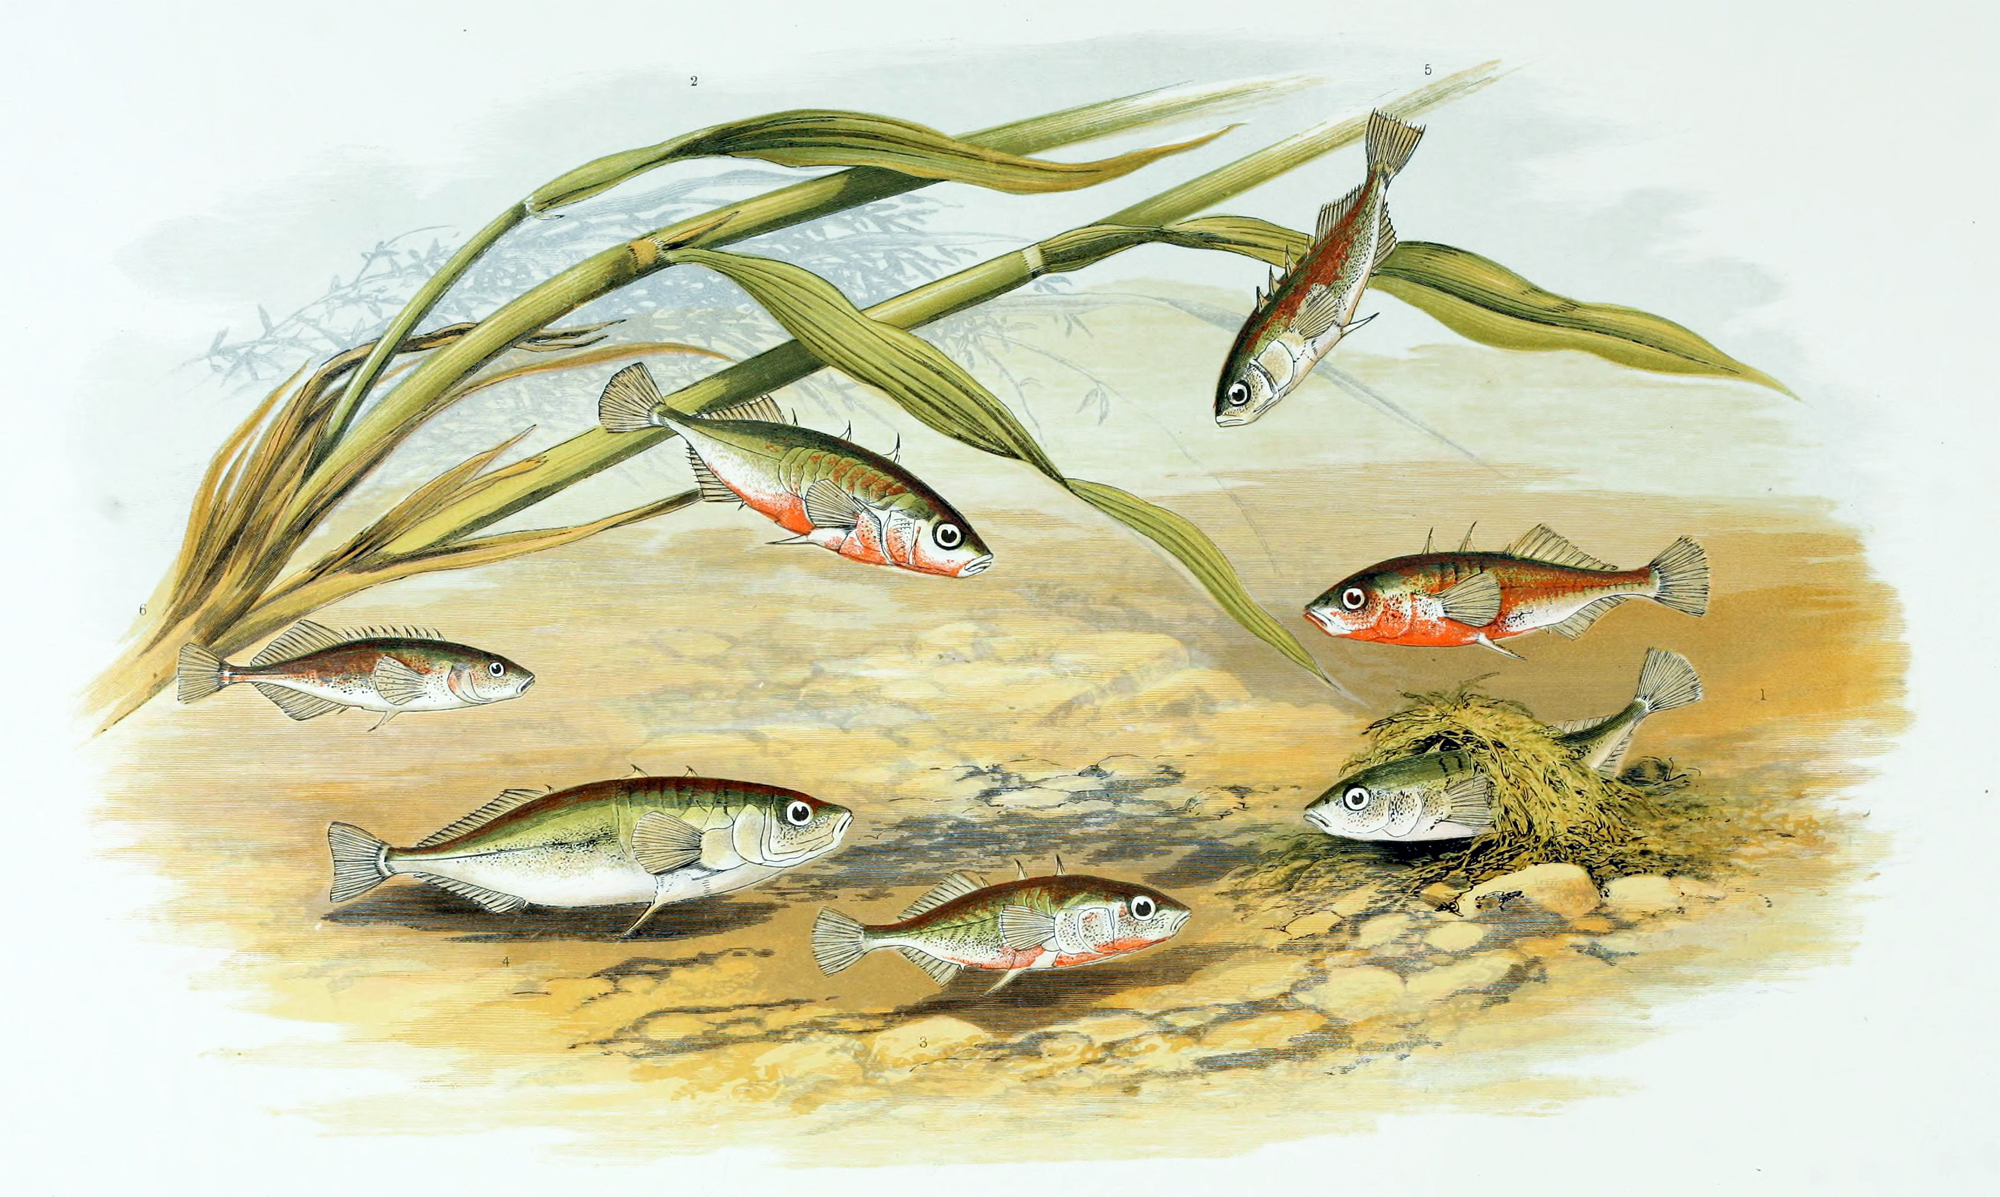
\includegraphics[width= \textwidth]{illustration_images/single_locus_selection/Stickleback/Gasterosteus_aculeatus_1879.jpg}
\end{center}
\caption{Freshwater threespine Stickleback ({\it
    G. aculeatus}). British fresh-water fishes. Houghton W 1879. BHL.} \label{fig:stickleback}
\end{marginfigure}
Marine threespine stickleback ({\it Gasterosteus aculeatus}) have
independently colonized and adapted to many freshwater lakes
as glaciers receded following the last ice age making them a
wonderful system for studying the genetics of adaptation. In marine
habitats most of the stickleback have armour plates to protect them
from predation, but freshwater populations repeatedly evolve the
loss of armour plates due to selection on an allele at the
Ectodysplasin gene (EDA).  This allele is found as a standing variant at very low frequency marine populations;
\citeauthor{Barrett:08} took advantage of this fact and collected and bred
a population of marine individuals carrying both the low- (L) and
completely- plated (C) alleles. The introduced the offspring of this
cross into four freshwater ponds and monitored genotype frequencies
\sidenote{The actual dynamics observed by \citeauthor{Barrett:08} are more complicated as in the very young fish selection reverses direction.}
over their life courses: 
\begin{center}
\begin{tabular}{lccc}
 & CC & LC & LL \\
Juveniles & 0.55 & 0.23 & 0.22\\
Adults     & 0.21 & 0.53 & 0.26\\
Juv./Adult ($W_{\bullet}/\Wbar$)  & 0.4 & 2.3 & 1.2 \\
rel. fitness ($W_{\bullet}/W_{12}$)  & 0.17 & 1.0 & 0.54 \\
\end{tabular}
\end{center}
The heterozygotes have increased in frequency dramatically in the
population as their fitness is more than double the mean fitness of
the population. We can also calculate the the relative fitness of each
genotype by dividing through by the fitness of the fitest genotype,
the heterozygote in this case (doing this cancels through
$\Wbar$). The relative fitness of the $CC$ is $\sim 1/5$ of the
heterozygote. Note that this calculation does not rely on the genotype frequencies being at their HWE in the juveniles.

\begin{question}
{\bf A} What is the frequency of the low-plated EDA allele ($L$) at the start
of the stickleback experiment? \\
{\bf B} What is the frequency in the adults? 

\end{question}


\begin{question}
You have been studying an annual wildflower for many generations with two color morphs orange and white. You have discovered that a single bi-allelic locus controls flower color, with the white allele being recessive. The pollinator of these plants is an almost blind bat, so individuals are pollinated at random with respect to flower color. Your population census of 200 individuals showed that the population consisted of 168 orange-flowered individuals, and 32 white-flowered individuals.\\
Heavy February rainfall creates optimal growing conditions for an
exotic herbivorous beetle with a preference for orange-flowered
individuals.  This year it arrives at your study site with a ravenous
appetite.  Only 50\% of orange-flowered individuals survive its wrath,
while 90\% of white-flowered individuals survive until the end of the
growing season.  \\
%Additionally, surviving orange flowered individuals produce 80 seeds on average, while surviving white-flowered individuals produce 100 seeds on average. 
{\bf A} What is the initial frequency of the white allele, and what do you
have to assume to obtain this?\\
{\bf B} What is the frequency of the white allele in the seeds forming the next generation?\\
\end{question}


The change in frequency from generation $t$ to $t+1$ is
\begin{equation}
\Delta p_t = p_{t+1} -p_{t}= \frac{w_{11} p_t^2 + w_{12} p_tq_t}{\wbar} - p_t. \label{deltap_dip1}
\end{equation}
To simplify this equation, we will first define two variables $\wbar_1$ and $\wbar_2$ as
\begin{eqnarray}
	\wbar_1 & = w_{11} p_t + w_{12} q_t, \\
	\wbar_2 & =  w_{12} p_t+ w_{22} q_t.
\end{eqnarray}
These are called the marginal fitnesses of allele $A_1$
and $A_2$, respectively. They are so called as $\wbar_1$ is the
average fitness of an allele $A_1$, i.e.\ the fitness of $A_1$ in a
homozygote weighted by the probability it is in a homozygote ($p_t$)
plus the fitness of $A_1$ in a
heterozygote weighted by the probability it is in a heterozygote ($q_t$).
We further note that the mean relative fitness can be expressed in terms of the marginal fitnesses as
\begin{equation}
	\label{eq:meanFitInTermsOfMargFit}
	\wbar = \wbar_1 p_t + \wbar_2 q_t,
\end{equation}
where, for notational simplicity, we have omitted the dependence of mean and marginal fitnesses on time.\\

We can then rewrite eqn.\ \eqref{deltap_dip1} using $\wbar_1$ and $\wbar_2$ as
\begin{equation}
	\Delta p_t = \frac{ (\wbar_1-\wbar_2)}{\wbar} p_t q_t.
	\label{deltap_dip2}
\end{equation}
The sign of $\Delta p_t$, i.e. whether allele $A_1$ increases of decreases
in frequency, depends only on the sign of $(\wbar_1-\wbar_2)$.
The frequency of $A_1$ will keep increasing over the generations so
long as its marginal fitness is higher than that of $A_2$,
i.e.\ $\wbar_1 > \wbar_2$, while if $\wbar_1 < \wbar_2$, the
frequency of $A_1$ will decrease. Note the similarity between eqn.\ \eqref{deltap_dip2} and the respective expression for the haploid model in eqn.\ \eqref{eq:deltap_haploid}. (We will return to the
special case where $\wbar_1 = \wbar_2$ shortly).\\

We can also rewrite \eqref{deltap_dip1} as
\begin{equation}
\Delta p_t =\frac{1}{2} \frac{p_tq_t}{\wbar} \frac{d \wbar}{dp},
\label{deltap_dip3}
\end{equation}
the demonstration of this we leave to the reader.
This form shows that the frequency of $A_1$ will increase ($\Delta p_t > 0$) if the mean fitness is an increasing function of the frequency of $A_1$ (i.e.\ if $\frac{d \wbar}{dp}>0$). On the other hand, the frequency of $A_1$ will decrease ($\Delta p_t < 0$) if the mean fitness is a decreasing function of the frequency of $A_1$ (i.e.\ if $\frac{d \wbar}{dp}<0$).
%This form shows that
%$\Delta p_t$ in increase if $\frac{d \wbar}{dp}>1$, i.e. increasing the
%frequency of $1$ increases the mean fitness, while the frequency of
%the allele with decrease if this increases the mean fitness of the
%population ($\frac{d \wbar}{dp}>1$).
Thus, although selection acts on
individuals, under this simple model, selection is acting to increase
the mean fitness of the population. \sa{The rate of this increase is proportional to
the variance in allele frequencies within the population ($p_tq_t$).}\\

\begin{question}
Show that eqns.\ \eqref{deltap_dip3} and \eqref{deltap_dip2} are
equivalent. (Trickier question.)\\
\end{question}

So far, our treatment of the diploid model of selection has been in terms of generic fitnesses $w_{ij}$. In the following, we will use particular parametrizations to gain insight about two specific modes of selection: directional selection and heterozygote advantage.

%%Selection coeffs in diploid model
\subsection{Diploid directional selection}
\begin{marginfigure}
\begin{center}
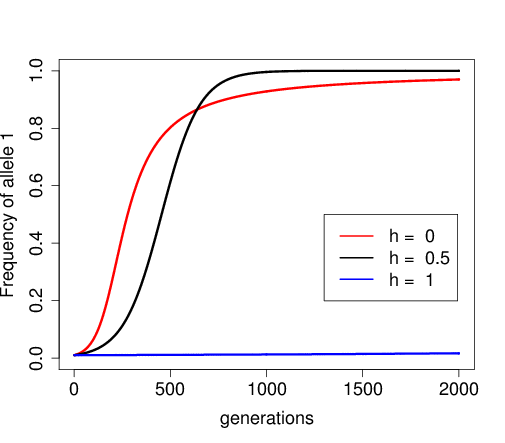
\includegraphics[width=\textwidth]{figures/simple_diploid_trajs.png}
\end{center}
\caption{The trajectory of the frequency of allele $A_1$, starting
  from $p_{0}=0.01$, for a selection coefficient $s=0.01$ and three
  different dominance coefficients. The recessive allele will
  eventually fix in the population, but it takes a long time.}
  \label{fig:diploid_traj}
\end{marginfigure}

Directional selection means that one of the two alleles always has higher marginal fitness than the other one. Let us assume that $A_1$ is the fitter allele, so that $w_{11} \geq w_{12} \geq w_{22}$, and hence $\wbar_1 > \wbar_2$\.
As we are interested in changes in allele frequencies, we \sa{may use} relative fitnesses. We parameterize the reduction in relative fitness in terms of a selection coefficient, similar to the
one we met in the haploid selection section, as follows:\\
\begin{center}
\begin{tabular}{lccc}
genotype & $A_1A_1$ & $A_1A_2$ & $A_2A_2$ \\
absolute fitness & $W_{11}$ & $ \geq W_{12} \geq$ & $W_{22}$ \\
relative fitness (generic) & $w_{11} = W_{11}/W_{11}$ & $w_{12} = W_{12}/W_{11}$ & $w_{22} = W_{22}/W_{11}$ \\
relative fitness  (specific) & $1$ & $1-sh$ & $1-s$. \\
\end{tabular}\\
\end{center}
Here, the selection coefficient $s$ is the difference in relative
fitness between the two homozygotes, and $h$ is the
dominance coefficient. \sa{For selection to be directional, we require that $0 \leq h \leq 1$ holds. The dominance coefficient allows us to move between two extremes. One is when $h = 0$, such that allele $A_1$ is fully dominant and $A_2$ fully recessive. In this case, the heterozygote $A_1A_2$ is as fit as the $A_1A_1$ homozgyote genotype. The inverse holds when $h = 1$, such that allele $A_1$ is fully recessive and $A_2$ fully dominant.}\\


%\gc{Yellow monkey flowers ({\it Mimulus guttatus}) have repeatedly adapted
%to the toxic soils found at copper mines throughout the Californian
%foothills in the past 150 years. Kevin Wright   }



%, of the $12$ and
%$22$ genotypes we will use selection coefficients $s_{12} \leq 0$ and
%$s_{22} \leq s_{12}$

We can then rewrite eqn.\ \eqref{deltap_dip2} as
\begin{equation}
\Delta p_t = \frac{p_ths + q_t s(1-h)}{\wbar}p_tq_t ,
\label{deltap_direct}
\end{equation}
where
\begin{equation}
\wbar_t = 1-2p_tq_t sh-q_t^2s.
\end{equation}\\


\begin{question}
Comparing the red ($h=0$) and black ($h=0.5$) trajectories in Figure \ref{fig:diploid_traj}, provide an explanation for why $A_1$ increases faster initially if $h=0$, but then approaches fixation more slowly compared to the case of $h=0.5$.
\end{question}

%%%% Another possible fox image
%%%  https://twitter.com/BioDivLibrary/status/1046777289416081408

%%%%%%%%%%%%%%%%%%%%%FOXSES
\begin{marginfigure}
\begin{center}
  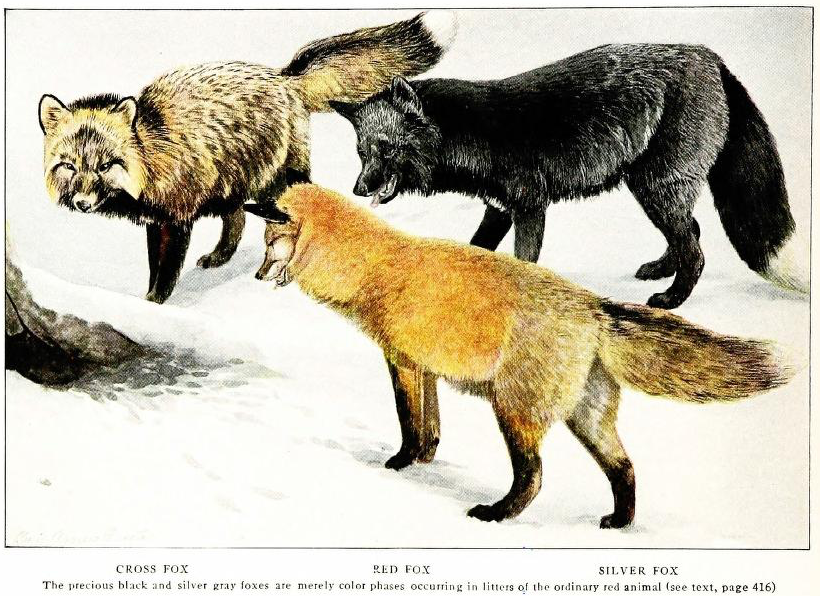
\includegraphics[width = \textwidth]{illustration_images/single_locus_selection/fox_morphs/fox_morphs_silver_cross.png}
\end{center}
\caption{Three colour morphs in red fox {\it V. vulpes}, cross, red,
  and silver foxes from left to right. From ``The
  larger North American mammals" Nelson, E.W., Fuertes, L.A. 1916.} \label{fig:Fox_morphs}
\end{marginfigure}
As an example of how dominance affects the trajectory of a real
polymorphism we'll consider an example from a colour polymorphism in
red foxes ({\it Vulpes vulpes}). There are three colour morphs of red foxes: silver, cross, and
red (see Figure \ref{fig:Fox_morphs}), with this difference primarily
controlled by a single polymorphism; with genotypes RR, Rr, rr respectively. The fur pelts of the silver morph
fetched three times the price for hunters compared to cross (a smoky red) and red
pelts, the latter two being seen as roughly equivalent in worth. Thus
the desirability of the pelts acts as a recessive trait, with much
stronger selection against the silver homozygotes.  As a
result of this price difference silver foxes were hunted more
intensely and declined as a proportion of the population in Eastern Canada, see Figure
\ref{fig:Fox_morph_freqs}, as documented by \citeauthor{elton:42},
from $16\%$ to $5\%$ from 1834 to 1937.
\begin{figure}
\begin{center}
  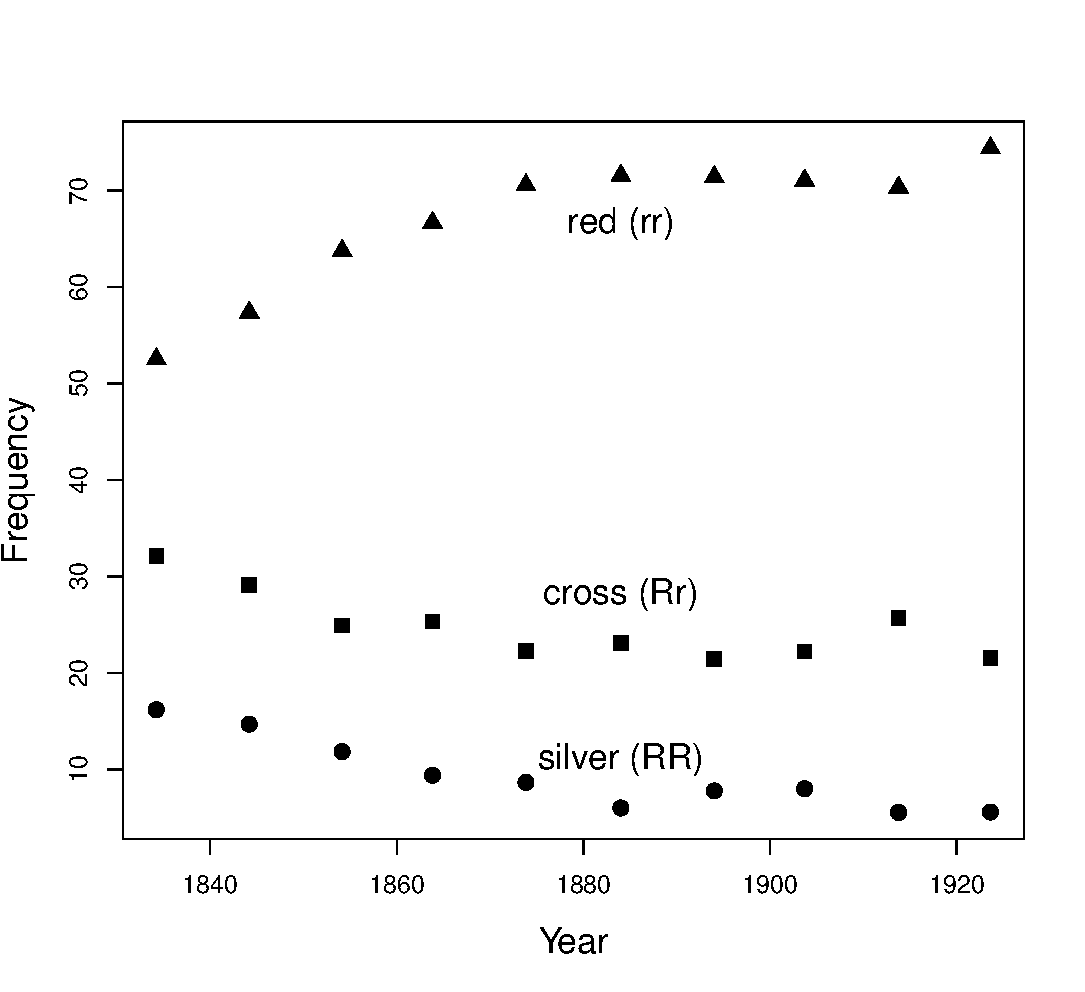
\includegraphics[width = \textwidth]{Journal_figs/single_locus_selection/silver_fox/fox_morph_freqs.pdf}
\end{center}
\caption{The frequency of red, cross, and silver fox morphs over the decades in Eastern Canada. These data are well described by recessive selection acting against the silver fox morph. Data from \citet{elton:42}, redrawn from \citet{Allendorf:09}.} \label{fig:Fox_morph_freqs}
\end{figure}
\citeauthor{haldane:42} reanalyzed these data and showed that they
were consistent with recessive selection acting against silver
morph alone. Note how the heterozygotes (cross) decline somewhat as a
result of selection on the silver homozygotes, but overall the R
allele is slow to respond to selection as it is `hidden' from
selection in the heterozygote state.

\graham{Add selection lines or get students to do that as an exercise.}


A special case is when $h = 0.5$. This case is the case of no dominance, as the interaction among alleles with respect to fitness is strictly additive. Then, eqn.\ \eqref{deltap_direct} simplifies to
\begin{equation}
	\Delta p_t = \frac{1}{2}\frac{s}{\wbar}p_tq_t .
	\label{deltap_add}
\end{equation}


If selection is very weak, i.e.\ $s \ll 1$, the denominator ($\wbar$) is close to $1$ and we have
\begin{equation}
	\Delta p_t = \frac{1}{2} s p_t q_t .
	\label{deltap_add_simpl}
\end{equation}
It is instructive to compare eqn.\ \eqref{deltap_add_simpl} to the respective expression under the haploid model. To this purpose, start from the generic term for $\Delta p_t$ under the haploid model in eqn.\ \eqref{eq:deltap_haploid} and set $w_1 = 1$ and $w_2 = 1-s$. Again, assume that $s$ is small, so that eqn.\ \eqref{eq:deltap_haploid} becomes $\Delta p_t = s p_t q_t$. Hence, if $s$ is small, the diploid model of directional selection without dominance is identical to the haploid model, up to a factor of $1/2$. That factor is due to the choice of the parametrisation; we could have set $w_{11} = 1$, $w_{12} = 1-s$, and $w_{22} = 1-2s$ in diploid model instead, in which case the agreement with the haploid model would be perfect.\\

From this analogy, we can borrow some insight we gained for the haploid model. Specifically, the trajectory of the frequency of allele $A_1$ in the diploid model without dominance follows a logistic growth curve similar to \eqref{eq:haploid_logistic growth}. Similarly, eqn.\ \ref{eq:fixTimeSimpl} for the haploid model suggests that in the diploid model without dominance it takes
\begin{equation}
	\tau \approx \frac{4}{s} \log(2N)  \label{eq:diploid_fix_time}
\end{equation}
generations for the favourable allele ($A_1$)
 to transit from its entry into the population ($p_0 =1/(2N)$)
to close to fixation ($p_{\tau} =1-1/(2N)$). Note again the difference
by a factor of 2 due to the choice of parametrization. Also, the total
number of alleles is $2N$ in the diploid model, rather than $N$, which
explains another factor of 2 in the argument of the logarithm. More
generally we can use this correspondance of the trajectory additive
diploid model to the haploid model to understand how quickly allele
frequencies should change given a selection coefficient between
arbitrary frequencies.\\


%\begin{tcolorbox} 
%\begin{question}
%An autosomal pesticide resistance allele is at 50\% frequency in a species of flies.  We stop using the pesticide, and within 20 years the frequency of the allele is 5\% in the new-born flies. There are two fly generations per year. Assuming that the allele affects fitness in an additive fashion, estimate the selection coefficient acting against homozygotes for the resistance allele.
%\end{question}
%\end{tcolorbox}


\subsection{Heterozygote advantage}
What if the heterozygotes are fitter than either
of the homozygotes? In this case, it is useful to parameterize the relative fitnesses as follows:\\
\begin{center}
\begin{tabular}{lccc}
	genotype & $A_1A_1$ & $A_1A_2$ & $A_2A_2$ \\
	absolute fitness & $w_{11}$ & $<w_{12}>$ & $w_{22}$ \\
	relative fitness (generic) & $w_{11}=W_{11}/W_{12}$ & $w_{12} = W_{12}/W_{12}$ & $w_{22} = W_{22}/W_{12}$ \\
	relative fitness (specific)  & $1-s_1$ & $1$ & $1-s_2$ \\
\end{tabular}\\
\end{center}

Here, $s_1$ and $s_2$ are the differences between the relative fitnesses
of the two homozygotes and the heterozygote. Note that to obtain
relative fitnesses we have divided
absolute fitness by the heterozygote fitness. We could use the
same parameterization as in the model of directional selection, but the reparameterization we have chosen here makes the math prettier.\\

In this case, when allele $A_1$ is rare, it is often found in a
heterozygous state and so it increases in frequency. However, when
allele $A_1$ is common, it is often found in the homozygote state, while
the allele $A_2$ is often found in the heterozygote state; it is
now $A_2$ that increases in frequency at the expense of allele
$1$. Thus, at least in the deterministic model, neither allele can
reach fixation and both alleles will be maintained as a balanced
polymorphism in the population at an equilibrium frequency.\\

We can solve for this equilibrium frequency by setting $\Delta p_t = 0$ in  eqn.\ \eqref{deltap_dip2}, 
i.e.\ $p_tq_t (\wbar_1-\wbar_2)=0$. Doing so, we find that there are three equilibria, all of which are stable. Two of them are not very interesting ($p=0$ or $q=0$), but the third one is the polymorphic equilibrium,  where
$\wbar_1-\wbar_2$ holds.
Using the parametrization above, we see that the marginal fitnesses of the two alleles are formally equivalent. Insertion of the selection coefficients $s_1$ and $s_2$ yields
\begin{equation}
	p_e = \frac{s_2}{s_1+s_2}
\end{equation}
for the equilibrium frequency of interest. This is also the frequency of $A_1$ at which the mean fitness of the population is maximised.\\

\paragraph{Underdominance.} Another case that is of potential interest is the case of fitness
underdominance, where the heterozygote is less fit than either of the
homozygotes. This can be parametrized as follows: \\
\begin{center}
\begin{tabular}{lccc}
	genotype & $A_1A_1$ & $A_1A_2$ & $A_2A_2$ \\
	absolute fitness & $w_{11}$ & $<w_{12}>$ & $w_{22}$ \\
	relative fitness (generic) & $w_{11}=W_{11}/W_{12}$ & $w_{12} = W_{12}/W_{12}$ & $w_{22} = W_{22}/W_{12}$ \\
	relative fitness (specific)  & $1+s_1$ & $1$ & $1+s_2$ \\
\end{tabular}\\
\end{center}

This case also permits three equilibria, $p=0$, $p=1$, and a
polymorphic equilibrium $p=p_U$. However,
now only the first two equilibria are stable, while the polymorphic
equilibrium is unstable. If $p<p_U$ then $\Delta p_t $ is negative
and allele $A_1$ will be lost, while if $p>p_U$, allele
$A_1$ will become fixed.\\

While such alleles might not spread within populations (if $p_U \gg
0$ and selection is reasonably strong), they are of interest in the study of speciation and hybrid
zones. That is because alleles $A_1$ and $A_2$ may have arisen in a
stepwise fashion, i.e.\ not by a single mutation, in separate
subpopulations. Now, heterozygote disadvantage will play a
potential role in species maintenance, if isolation of the subpopulations is not complete.\\

\begin{tcolorbox} 
\begin{question}
You are studying the polymorphism that affects flight speed in butterflies. The polymorphism does not appear to affect fecundity.  Homozygotes for the B allele are slow in flight and so only 40\% of them survive to have offspring. Heterozygotes for the polymorphism (Bb) fly quickly and have a 70\% probability of surviving to reproduce. The homozygotes for the alternative allele (bb) fly very quickly indeed, but often die of exhaustion, with only 10\% of them making it to reproduction.  \\
{\bf A)} What is the equilibrium frequency of the B allele?\\
{\bf B)} Calculate the marginal fitnesses of the B and the b allele at
the equilbrium frequency. 
\end{question}
\end{tcolorbox}

\paragraph{Diploid fluctuating fitness}
We would like to think about the case where the diploid absolute fitnesses
are time-dependent. The three genotypes then have fitnesses
$w_{11,t}$, $w_{12,t}$, and $w_{22,t}$ in generation $t$. However,
this case is much less tractable than the haploid case, as segregation
makes it tricky to keep track of the genotype frequencies.  
We can make some progress and gain some intuition by thinking about
how the frequency of allele $A_1$ changes when it is rare.\\
\graham{Haldane and Jayakar (1963) }

% (This argument is originally due to Haldane and J. )\\

Selection pressures clearly fluctuate over time, how does this affect
the dynamics of polymorphisms. Two examples of polymorphisms
fluctuating in frequency in response to temporally-varying selection
are shown in Figure \ref{fig:Droso_fluct}; thanks to the short
lifespan of {\it Drosophila} we can see seasonally-varying selection. The first is an inversion
allele in {\it Drosophila pseudoobscura}, in {\it D. pseudoobscura}
populations. Throughout western North America two orientations of the
chromosome, two inversion alleles, exist: the Chiricahua and Standard
alleles. \graham{Add figure of het.} \citeauthor{wright:46}
\graham{need earlier Dob. ref IX} investigated their frequency over
four years at a number of locations, and found that their frequency
fluctuated systematically over the seasons in response to
selection. Our second example is an insertion-deletion polymorphism in
the Insulin-like Receptor gene. \citeauthor{paaby:14} tracked the
frequency of this allele over a number of seasons, and found it
oscillated over the seasons. She and her coauthors also determined that these alleles had large effects on
traits such as developmental time and fecunity, which could mediate
the maintainance of this polymorphism through life-history trade-offs.

\begin{figure}
\begin{center}
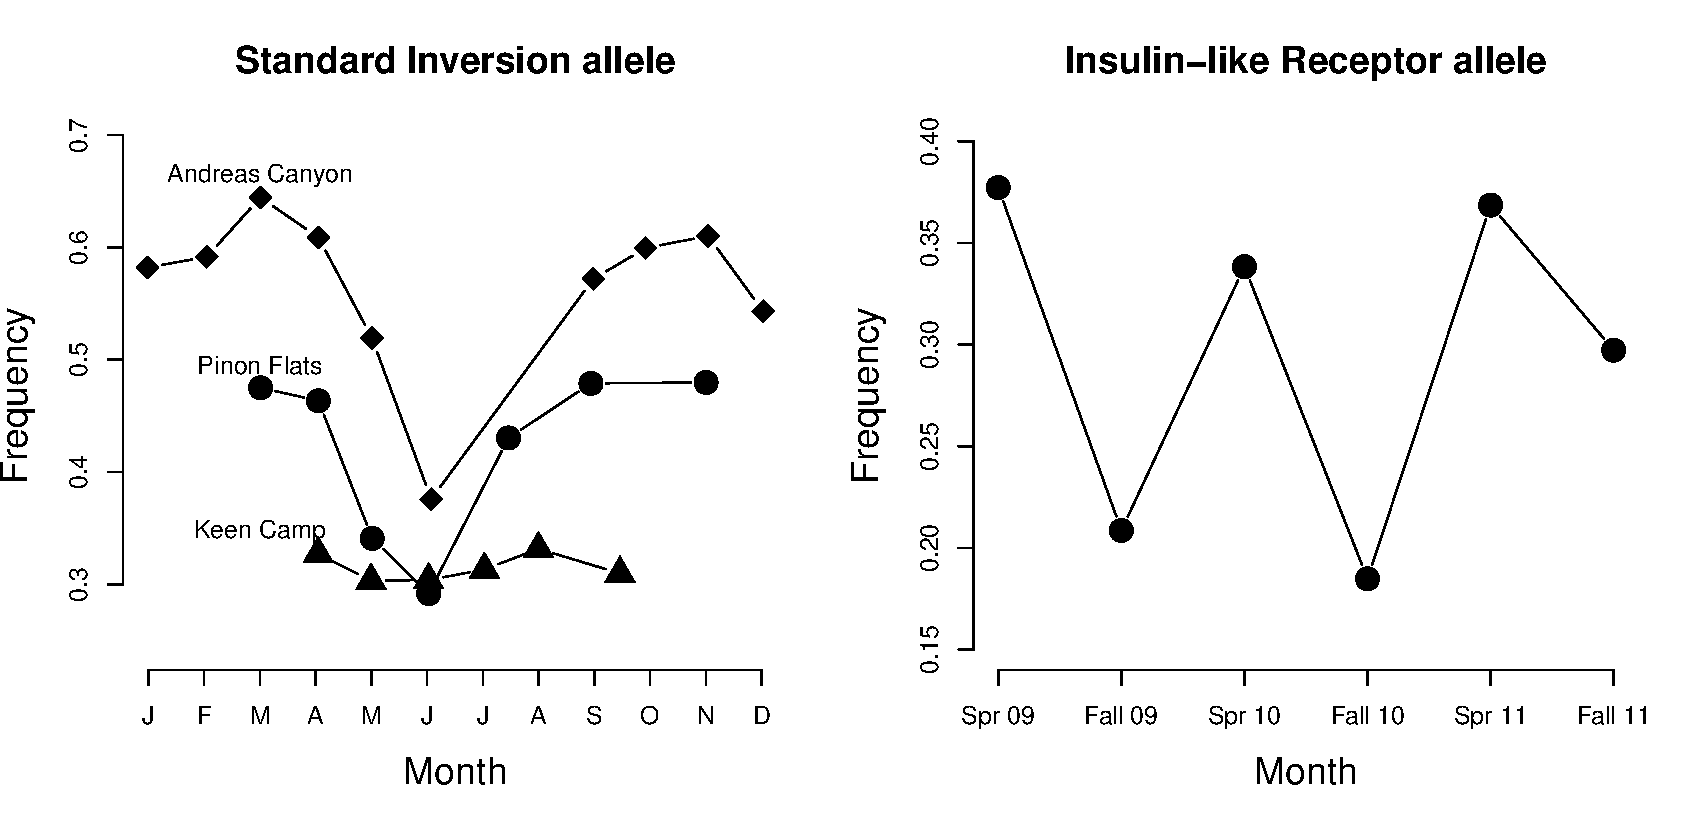
\includegraphics[width=\textwidth]{Journal_figs/single_locus_selection/temporal_Droso_freq/temporal_Droso_freq.pdf}
\end{center}
\caption{  } \label{fig:Droso_fluct} 
\end{figure}

When $A_1$ is rare, i.e.\ $p_t \ll 1$, its frequency in the next
generation \eqref{pgen_dip} can be approximated as
\begin{equation}
p_{t+1} \approx \frac{w_{12}}{\wbar} p_t.
\end{equation}
To obtain this, we have ignored the $p_{t}^2$ term and assumed that $q_t \approx 1$ in the numerator.
Following a similar argument to approximate $q_{t+1}$, we can write
\begin{equation}
	\frac{p_{t+1}}{q_{t+1}} = \frac{w_{12,t}}{w_{22,t}}  \frac{p_{t}}{q_{t}}.
\end{equation}
Then, starting from out from $p_0$ and $q_0$ in generation $0$, $t+1$
generations later, we have
\begin{equation}
	\frac{p_{t+1}}{q_{t+1}} = \left( \prod_{i=0}^{t-1} \frac{w_{12,i}}{w_{22,i}}  \right) \frac{p_{0}}{q_{0}}.
\end{equation}
From this, we can see, following our haploid argument from above, that
the frequency of allele $A_1$ will increase when rare only if
\begin{equation}
	\frac{\sqrt[t]{\prod_{i=0}^{t-1}w_{12,i}}}{\sqrt[t]{\prod_{i=0}^{t-1}w_{22,i}}}>1 \label{geometric_1wins},
\end{equation}
i.e. if the heterozygote has higher geometric mean fitness than the $A_2A_2$ homozygote.\\

The question now is, whether allele $A_1$ will approach fixation in the population,
or whether there are cases in which we can obtain a balanced polymorphism. To investigate that, we can simply repeat our analysis for $q \ll 1$, and see that in that case
\begin{equation}
	\frac{p_{t+1}}{q_{t+1}} = \left( \prod_{i=0}^{t-1} \frac{w_{11,i}}{w_{12,i}}  \right) \frac{p_{0}}{q_{0}}.
\end{equation}
Now, for allele $A_1$ to carry on increasing in frequency and to
approach fixation, the $A_1A_1$ genotype has to be
out-competing the heterozygotes. For allele $A_1$ to approach
fixation, we need the geometric mean of $w_{11,i}$ to be greater than the
geometric mean fitness of heterozygotes ($w_{12,i}$).
At the same time, if heterozygotes have higher geometric mean fitness than
the $A_1A_1$ homozygotes, then the $A_2$ allele will increase in frequency when it is rare.
Therefore, a balanced polymorphism can result when the heterozygote
has higher geometric fitness than either of the homozygotes.\\

%\begin{equation}
%\frac{\sqrt[t]{\prod_{i=0}^{t}w_{11,i}}}{\sqrt[t]{\prod_{i=0}^{t}w_{22,i}}}>1
%\end{equation}
%implying that our $11$ homozygotes have to have higher geometric mean
%fitness than our heterozygotes.
%\begin{equation}
%\frac{\sqrt[t]{\prod_{i=0}^{t}w_{11,i}}}{\sqrt[t]{\prod_{i=0}^{t}w_{22,i}}}<1  \label{geometric_2wins}
%\end{equation}
%(satisfying both \eqref{geometric_1wins} and
%\eqref{geometric_2wins}).

Intriguingly, we can have a balanced polymorphism even if the
heterozygote is never the fittest genotype in any generation, if the heterozygotes
has a higher geometric mean fitness than either of the homozygotes. In this case, the polymorphism will remain balanced in the population,
despite the fact that the heterozygote is never the fitest genotype.

%To see
%this, consider the simple example, where there are two environments
%alternate from generation to generation:\\
%\begin{tabular}{lccc}
%genotype & $A_1A_1$ & $A_1A_2$ & $A_2A_2$ \\
%relative fitness in environment A & $w_{11,A}$ & $>w_{12,A}>$ & $w_{22,A}$ \\
%relative fitness in environment B  & $w_{11,B}$ & $<w_{12,B}<$ & $w_{22,B}$ \\
%Geometric mean fitness & $w_{11,B}$ & $<w_{12,B}>$ & $w_{22}$ \\
%\end{tabular}\\


\begin{tcolorbox}
\begin{question}
Consider a plant population found in one of two different environments each
generation. These occur randomly, $\nicefrac{1}{3}$ of time the population
experiences the dry environment and with probability $\nicefrac{2}{3}$ it
experiences the wet environment Y. The Absolute Fitnesses
are as follows:
\begin{center}
\begin{tabular}{cccc} 
Environment & AA & Aa & aa \\
\hline \\
Wet. & 6.25 & 5.0 & 3.75 \\
Dry & 3.85 & 5.0 & 6.15\\
\end{tabular}
\end{center}
{\bf A)} Show whether the equilibrium frequency of A will be $0$, $1$, or in between.\\
{\bf B)} If the probabilities of wet and dry environments were equal,
i.e., 0.5 how would your conclusion change?\\
(HINT: Lets write $w_{AA,\text{dry}}$ and $w_{AA,\text{wet}}$ for the
fitnesses of the AA homozygote in the two environments. Then if the
two environments are equally common $\prod_{i=0}^{t}w_{AA,i} \approx w_{AA,\text{dry}}^{\nicefrac{t}{2}}
w_{AA,\text{wet}}^{\nicefrac{t}{2}}$ for large values of $t$.)
%> (6.25)^(1/3)*(3.85)^(2/3);(5)^(1/3)*(5)^(2/3);(3.75)^(1/3)*(6.15)^(2/3)
%[1] 4.524812, 5, 5.215074
% (6.25)^(1/2)*(3.85)^(1/2);(5)^(1/2)*(5)^(1/2);(3.75)^(1/2)*(6.15)^(1/2)
% 4.905354, 5, 4.802343
\end{question}
\end{tcolorbox}

\begin{tcolorbox} 
\begin{question}
OPTIONAL trickier question.\\
Imagine a randomly-mating population of hermaphrodites. In this
population a derived allele (D) segregates that distorts transmission
in its favour over the ancestral allele (d) in the production of all
the gametes of heterozygotes. The drive leads to a fraction $r$ of the gametes
of heterozygotes (D/d) to carry the D allele ($r>0.5$). The D allele
causes viability problems in the homozygote state such that the
relative fitnesses are $w_{dd}=1$, $w_{Dd}=1$, $w_{DD}=1-e$. The allele
is currently at frequency p in the population at birth. Assuming that the
population is very large and no mutation occurs:\\
{\bf A)}	What is the frequency of the D allele in the next generation, before selection has had a chance to act?\\
{\bf B)}	What conditions do you need for a polymorphic equilibrium to be maintained? At what is the equilibrium frequency of this balanced polymorphism?\\
{\bf C)}	Imagine the cost of the driver were additive
$w_{dd}=1$, $w_{Dd}=1-e$, $w_{DD}=1-2e$. Under what conditions can the driver invade the population? Can a polymorphic equilibrium be maintained?
\end{question}
\end{tcolorbox}

\subsection{Mutation--selection balance}
%</source-file>
Mutation is constantly introducing new alleles into the
population. Therefore, variation can be maintained within a
population not only if selection is balancing (e.g.\ through heterozygote advantage or fluctuating selection over time, as we have seen in the previous section), but also due to a balance between
mutation and selection\cite{Haldane:37}. A case of particular interest is when mutation introduces deleterious alleles and selection acts against these alleles. To study this balance, we return to the model of directional selection, where allele $A_1$ is advantageous, i.e.
\begin{center}
\begin{tabular}{lccc}
genotype & $A_1A_1$ & $A_1A_2$ & $A_2A_2$ \\
absolute fitness & $W_{11}$ & $ \geq W_{12} \geq$ & $W_{22}$ \\
relative fitness & $w_{11}=1$ & $w_{12}=1-sh$ & $w_{22}=1-s$. \\
\end{tabular}\\
\end{center}

For a start, we consider the case where allele $A_2$ is not
completely recessive ($h>0$), so that the heterozygotes suffer at least some disadvantage. We denote by $\mu = \mu_{1\rightarrow2}$ the  mutation rate per generation from $A_1$ to the deleterious allele $A_2$, and assume that there is no reverse mutation ($\mu_{2\rightarrow1} = 0$).  Let us assume that selection against $A_2$ is relatively strong compared to the mutation rate, so that it is justified to assume that $A_2$ is always rare, i.e.\ $q_t = 1-p_t \ll 1$. Compared to previous sections, for mathematical clarity, we also switch from following the frequency $p_t$ of $A_1$ to following the frequency $q_t$ of $A_2$. Of course, this is without loss of generality. The change in frequency of $A_2$ due to selection can be written as
\begin{equation}
	\Delta_S q_t = \frac{\wbar_2 - \wbar_1}{\wbar} p_t q_t  \approx  -hs q_t.
	\label{eq:dirSelApprox}
\end{equation}
This approximation can be found by assuming that $q^2 \approx 0$, $p \approx 1$,
and that $\wbar \approx w_1$. \sa{All of these assumptions make sense if $q \ll 1$. From eqn.\ \eqref{eq:dirSelApprox} we see that selection acts to reduce the frequency of $A_2$ (as both $h$ and $s$ are positive), and it does so geometrically across the
generations. That is, if the initial frequency of $A_2$ is $q_0$, then its frequency at time $t$ is approximately 
\begin{equation}
	q_t = q_0 (1 - hs)^t.
	\label{eq:dirSelExplApprox}
\end{equation}

We will now consider the change in frequency induced by mutation. Recalling that $\mu$ is
the mutation rate from $A_1$ to $A_2$ per generation, the frequency of $A_2$ after mutation
\begin{equation}
	q^{\prime} =  \mu p_t + q_t = \mu(1 - q_t) + q_t.
\end{equation}
Assuming that $\mu \ll 1$ and that $q \ll 1$, the change in the
frequency of allele $A_2$ due to mutation ($\Delta_M q_t$) can be approximated by
\begin{equation}
	\Delta_M q_t = q^{\prime} - q_t =  \mu.
	\label{eq:mutApprox}
\end{equation}
Hence, when $A_2$ is rare and the mutation rate is low, mutation acts to linearly increase the frequency of the deleterious allele $A_2$.\\

If selection is to balance deleterious mutation, their combined effect over one generation has to be zero. Therefore, to find the mutation--selection equilibrium, we set
\begin{equation}
	\Delta_M q_t + \Delta_S q_t = 0,
\end{equation}
insert eqns. \eqref{eq:dirSelApprox} and \eqref{eq:mutApprox}, and solve for $q$ to obtain
\begin{equation}
	q_e = q_t = \frac{\mu}{hs}.
	\label{eqn:mut_sel_bal}
\end{equation}
We see that the frequency of the deleterious allele $A_2$ is balanced at the mutation rate ($\mu$) divided by
the reduction in relative fitness in the heterozygote ($hs$).}\\

It is worth pointing out that the fitness of the $A_2A_2$ homozygote
has not entered this calculation, as $A_2$ is so rare that it is hardly ever found in the 
homozygous state. Therefore, if $A_2$ has any deleterious effect
in a heterozygous state (i.e.\ if $h>0$) it is this effect that determines the
frequency at which $A_2$ is maintained in the population. Also, note that by
writing the total change in allele frequency as $\Delta_M q_t + \Delta_S q_t
$ we have implicitly assumed that we can ignore terms of order $\mu
\times s$. That is, we have assumed that there is no interaction between mutation and selection. We can do so as we assumed that both $\mu$ and $s$ are small.\\


If an allele was truly recessive (although few likely are), we have $h=0$, and
so eqn.\ \eqref{eqn:mut_sel_bal} is not valid. However, we can make an argument similar to the one above to show
that, for truly recessive alleles,
\begin{equation}
	q_e = \sqrt{\frac{\mu}{s}}.
\end{equation}

\begin{marginfigure}
\begin{center}
  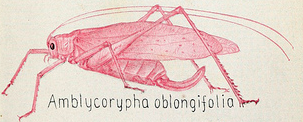
\includegraphics[width = \textwidth]{Journal_figs/single_locus_selection/mutation_selection_balance/Pink_Katydid.png}
\end{center}
\caption{Oblong-winged katydid. Field book of insects. Lutz,
  F.E. 1918.} \label{fig:katydid}  %https://www.flickr.com/photos/biodivlibrary/6244366674/in/photolist-avN1Eo-oryMQJ-otszkE-owcT1v-rmioFJ-rshxSS-otehvW-r94w4a-odY9oG-ouGyrw-ormnow-otADXZ-ce8krE-ouviqy-rsgo6D-owjZfG-otERD9-osGcMG-tFBjpS-ovagk4-vNj4qo-raPuoW-odiS3R-r71XYf-ovhSyW-roAbgX-otSMZn-oteYxg-owtP1B-ouk7tq-rsgj5c-roAhrc-otwafC-r94wYr-wX5186-tBBz3o-ouJWQD-oe1erd-ovhT8d-r72RMs-otTfyG-oujQ9m-vdVLQQ-rsnUL8-oderxh-ov94Ci-otABpx-odf6U7-xeyTGn-oukYY8
\end{marginfigure}

\begin{question}
Oblong-winged katydids ({\it Amblycorypha oblongifolia}) are usually
% these are actually false katydid
green. However, some are bright pink, thanks to a erythrism
mutation (a nice example of an early Mendelian reasoning in a wonderful
titled paper\cite{Wheeler:07}). This condition is thought to be due to
a dominant mutation (\citeauthor{Crew:13}). Assume that roughly
one in ten thousand is bright pink and that the mutation rate at the
gene underlying this condition is $10^{-5}$. What is the relative fitness of heterozygotes for the pink mutation? 
\end{question}


\paragraph{The genetic load of deleterious alleles}
What effect do such deleterious mutations at mutation--selection balance have on the population? It is common to express this effect in terms of a reduction of the mean relative fitness of the population. For a single site at which a deleterious mutation is segregating at $q_e = \mu/(hs)$, the mean relative fitness is reduced to
\begin{equation}
	\wbar = 1- 2p_e q_e hs - q_e^2s \approx 1-2\mu.
\end{equation}
Somewhat remarkably, the drop in mean fitness due to a site segregating
at mutation--selection balance is independent of the selection coefficient against the
heterozygote; it depends only the mutation rate. Note that this applies only if the mutation is not totally recessive, i.e.\ if $h > 0$.

A reduction of $1 - 2\mu$ is very small, given that the
mutation rate of a gene is likely $<10^{-5}$. However, if there are many loci
segregating at mutation--selection balance, this can accumulate to a substantial so-called
genetic load, and a major cause of variation in fitness-related traits
among individuals. For example, the human genome contains over twenty
thousand genes, and many other functional regions, the vast majority
of which will be subject to purifying selection against mutations that
disrupt their function. In humans most loss of function (LOF) variants, which severely
disrupt a protein-coding gene, are found at low frequencies. However, each human genome typically carries over
hundred LOF variants \citep{macarthur:12,lek:16}. Not every LOF allele will be
deleterious, some could be advantagous, but the combined load of these
LOF must on average lower our fitness, otherwise selection wouldn't be
removing them from the population. Each one of us
carries a unique set of these LOF alleles.. We differ slightly in how
many of these alleles we carry. For example Figure \ref{fig:LOF} shows
the distribution of number of LOF alleles carried by 769 individuals
of Dutch ancestry. The individuals who carry fewer of these LOF
alleles will on average have higher fitness than those individuals
with more. We don't let know how much lower the fitness of these
individuals is, nor how most of these alleles manifest their fitness
consequences through disease and other mechanisms.  


\begin{marginfigure}
\begin{center}
  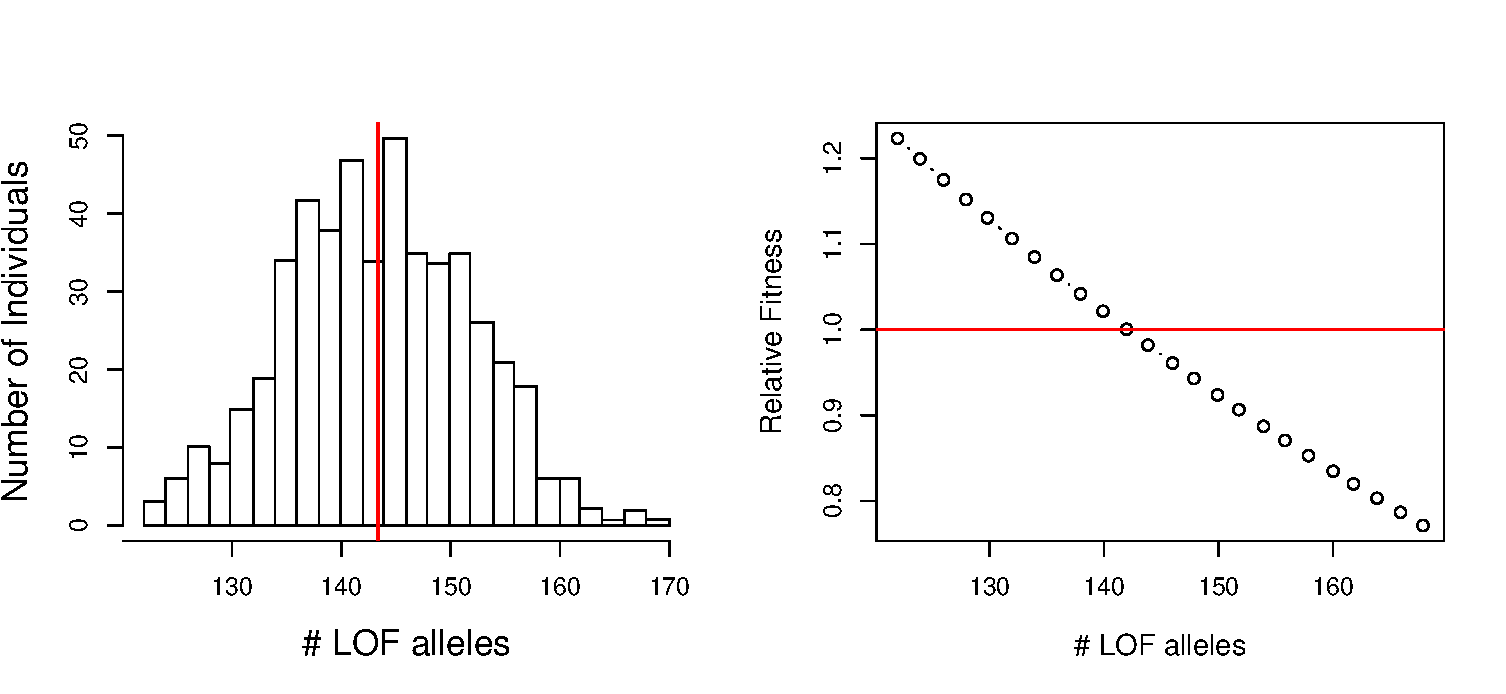
\includegraphics[width = \textwidth]{Journal_figs/single_locus_selection/LOF_variants/Neatherlands_LOF_variants.pdf}
\end{center}
\caption{The distribution of LOF alleles in 769 individuals from the
  Genome of the Netherlands project. Redrawn from
  \citeauthor{francioli:14}. The average individual carries 144 LOF
  alleles. } \label{fig:LOF} 
\end{marginfigure}


%\begin{question}


%\begin{tcolorbox} 
%\begin{question}
%You are studying an outbred population of mice living in a farmer’s field. Mutations occur at a gene called nurseryrhyme that cause a totally recessive form of blindness. These blind mice do not survive to reproduce as the farmer’s wife cuts off their tail (and other bits) with a carving knife. 
%Surveying the field for baby mice you find that 3 in ten thousand mice are blind.\\
%{\bf A} Assuming that the population mates at random, what is the mutation
% rate of blindness causing alleles?\\
%{\bf B} Following more careful study you now find that there is actually a $20
%\%$ reduction in the viability of heterozygotes for these
%mutations. What would you now estimate as the mutation rate for this
%gene?  
%{\bf C)} Explain how and why your answers differ?
%\end{question}
%\end{tcolorbox}

%B) You look at family of outbred mice. You find that one of the mice in the family is blind, what is the probability that its 1st cousin is also blind?

%C) In another isolated field on the farm, there is a high rate of inbreeding among the mice. The farmer’s wife also carries out her cruel carving knife policy in this field as well. Do you expect to the underlying blindness mutations to be at a higher or low rate in this second field than the first field? Briefly explain your answer.


\subsection{Inbreeding depression}
All else being equal, eqn.\ \eqref{eqn:mut_sel_bal} suggests that mutations that have a smaller effect in the
heterozygote can segregate at higher frequency under mutation--selection balance. As a consequence, alleles that have
strongly deleterious effects in the homozygous state can segregate at
low frequencies in the population, as long as they do not have too 
strong a deleterious effect in heterozygotes. Thus, outbred populations may have many
alleles with recessive deleterious effects segregating within them.
\begin{question}
Assume that a deleterious allele has a relative fitness $.99$ in
heterozygotes and a relative fitness $0.2$. Assuming that the
deleterious allele is at a frequency $10^{-3}$ at birth the
genotype frequencies follow from HWE:\\
{\bf A)} What is the average fitness of an individual in the population
due to this allele? \\
 {\bf B)} What is the fitness of the child of a full-sib mating? \\
\end{question}
One consequence of this is that inbred individuals from usually outbred
populations may have lower fitnesses than outbred
individuals.  In typically outbred populations, the mean fitness of individuals
decreases with the inbreeding coefficient, i.e.\ this so-called inbreeding depression
is a common observation. This is wide-spread observation, dating back to systematic
surveys of inbreeding depression by \citeauthor{darwin:1876}.
Inbreeding depression is likely as primarily a consequence of being homozygous at many loci for
alleles with recessive deleterious effects.
\begin{marginfigure}
\begin{center}
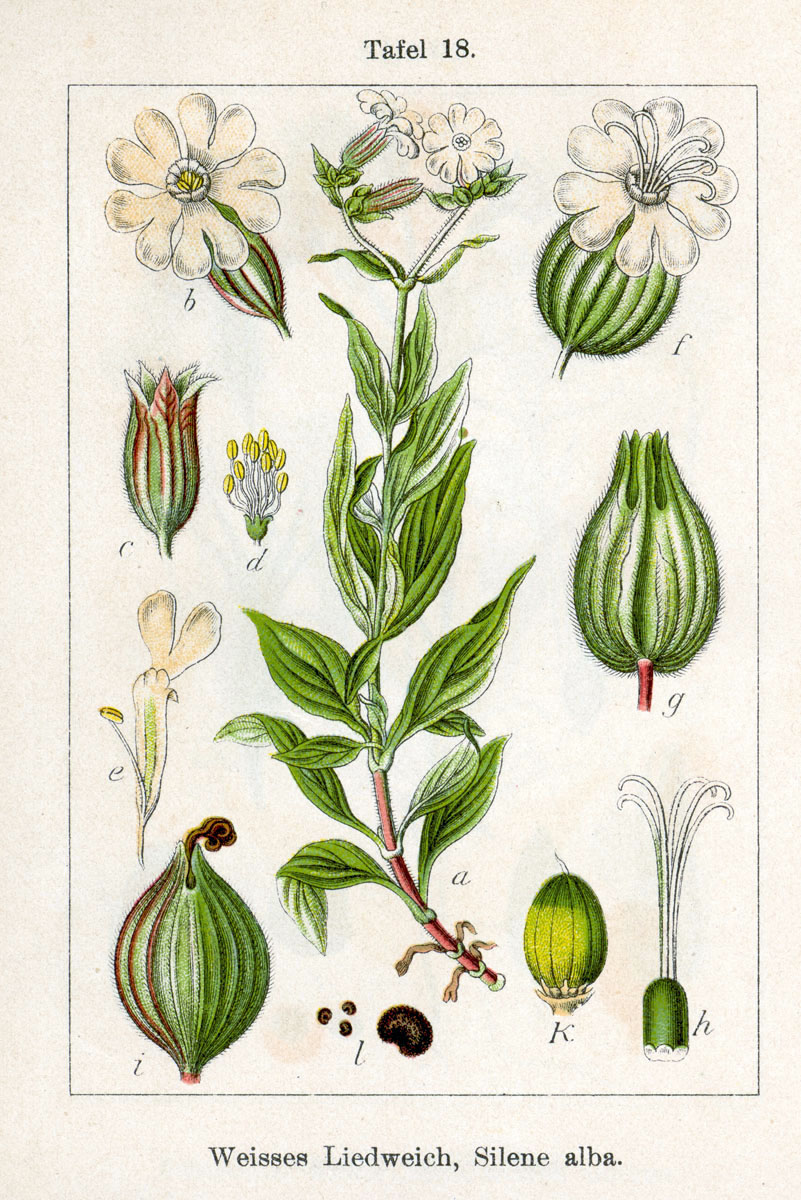
\includegraphics[width = \textwidth]{illustration_images/single_locus_selection/Silene_inbreeding_dep/Silene_latifolia_Sturm18.jpg}
\end{center}
\caption{  White
campion  ({\it S. latifolia}) } \label{fig:Silene} 
\end{marginfigure}

One example of inbreeding
depression is shown in Figure \ref{fig:Silene_inbreeding}.  White
campion ({\it Silene latifolia}) is a dioecious flowering plant, dioecious means that the males and females are
separate individuals. \citeauthor{richards:00} performed crosses to
create offspring who were outbred, the offspring of half-sibs,
full-sibs, and of two generations of full-sib mating. He measured
their germination success, which is plotted in Figure \ref{fig:Silene_inbreeding}.


\begin{figure}
\begin{center}
  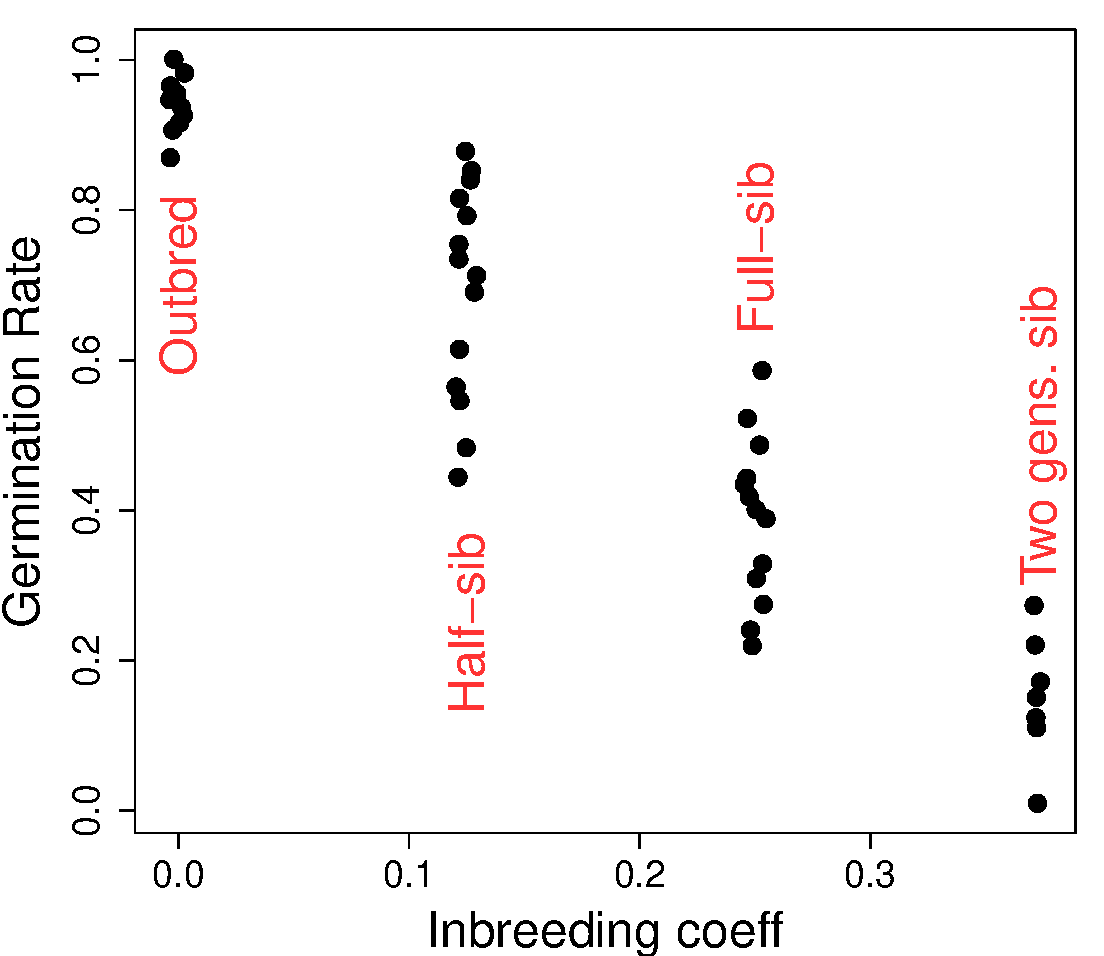
\includegraphics[width = \textwidth]{Journal_figs/single_locus_selection/Silene_inbreeding_Richards/Silene_inbreeding_depression.pdf}
\end{center}
\caption{Data showing inbreeding depression over different degrees of
  inbreeding in {\it S. latifolia}. Each point is the mean seed germination rates for different
  family crosses.  Redrawn from \citeauthor{richards:00}. } \label{fig:Silene_inbreeding} 
\end{figure}

\graham{Add theory line?}

\paragraph{Purging the inbreeding load.}
Populations that regularly inbreed over sustained periods of time
are expected to partially purge this load of deleterious
alleles. This is because such populations have exposed many of these alleles
in a homozygous state, and so selection can more readily remove these alleles
from the population.

If the population has sustained inbreeding, such that individuals in the population have an inbreeding
coefficient $F$, deleterious alleles at each locus will find a
new equilibrium frequency. Assuming the model of mutation-selection
model, with this inbreeding is, the new equilbrium frequency is 
\begin{equation}
	q_e = \frac{\mu}{\big( h(1-f) + f \big) s}
\end{equation}
Note how the frequency of the deleterious allele is decreased due to
the allele now being expressed, and therefore exposed to selection, in
homozygotes due to inbreeding.  


\newpage
\subsection{Migration--selection balance}
Another reason for the persistence of deleterious alleles in a
population is that there is a constant influx of maladaptive alleles
from other populations where these alleles are locally adapted.
This seems unlikely to be as broad an explanation for the
persistence of deleterious alleles genome-wide as mutation-selection
balance. However, a brief discussion of such alleles is worthwhile as
it helps to inform our ideas about local adaptation.\\


\gc{Adaptation can occur over a range of geographic scales.}

Adaptation can potentially occur on much finer geographic scales
from kilometers down to meters in some species. On such scales
dispersal is surely rapidly moving alleles between environments, but
the adaptation is maintained by the continued action of selection. An
example of adaptation at fine-scales is shown in Figure
\ref{fig:Zinc_mine}.. \gc{Jain and
  Bradshaw} studied the patterns of heavy-metal resistance in plants
on mine tailings and in nearby meadows, a set of classic studies of 
\begin{figure}
\begin{center}
  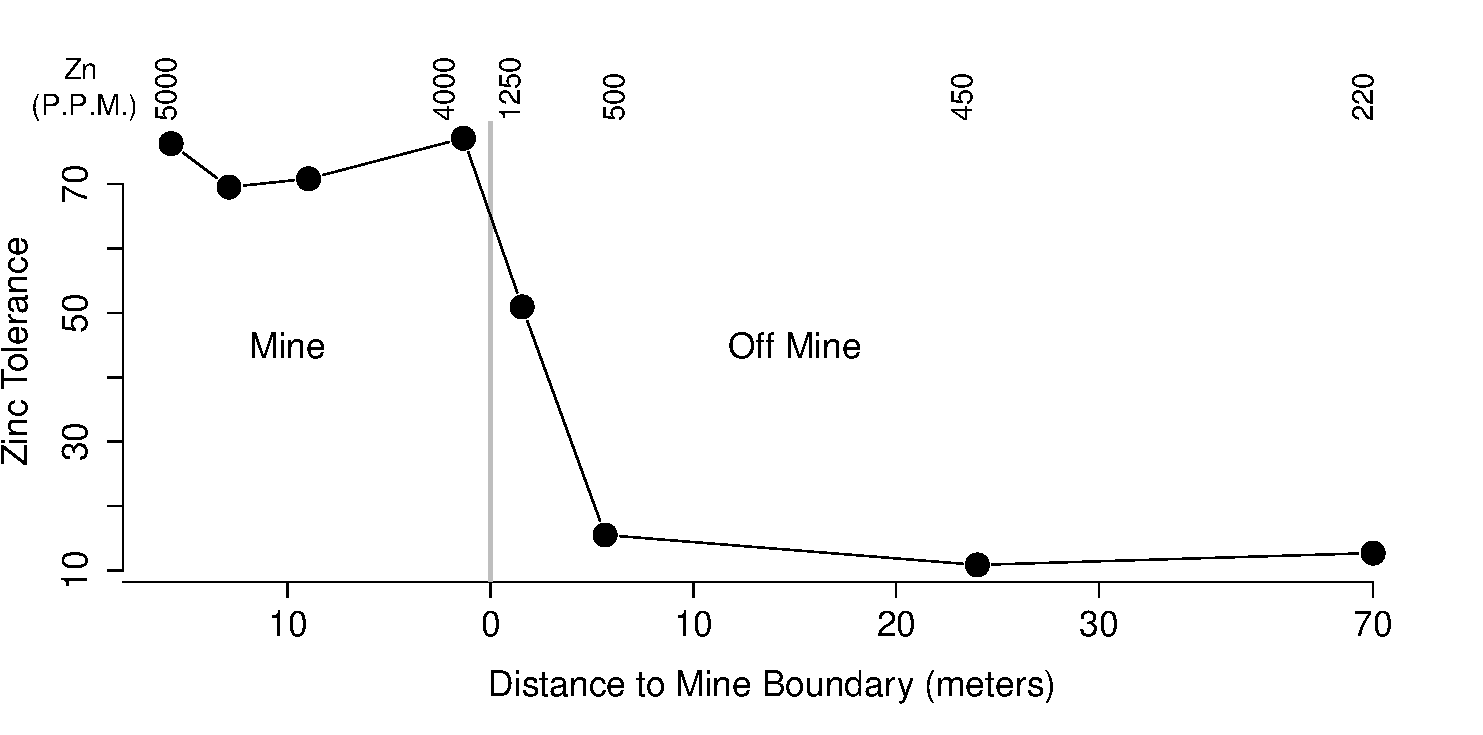
\includegraphics[width = \textwidth]{Journal_figs/single_locus_selection/Anthoxanthum_mines_Jain_Bradshaw/Anthoxanthum_zinc.pdf}
\end{center}
\caption{Data showing the Zinc tolerance of {\it Anthoxanthum
odoratum} on and off of the Trelogan
Mine, Flintshire, North Wales. } \label{fig:Zinc_mine} 
\end{figure}




As a first pass at this lets consider a haploid two allele model with
two different populations, where the relative fitnesses of our alleles
are as follows
\begin{center}
\begin{tabular}{c|cc}
allele & $1$ & $2$ \\
\hline
population 1 & 1 & 1-s \\
population 2 & 1-s & 1 \\
\end{tabular}
\end{center}
As a simple model of migration lets suppose within a population a
fraction of $m$ individuals are migrants from the other population,
and $1-m$ individuals are from the same deme.\\

To quickly sketch a solution to this, we'll set up a situation analogous
to our mutation-selection balance model. To do this let's assume that selection is strong compared to migration ($s \gg m$) then allele
$1$ will be almost fixed in population $1$ and allele $2$ will be
almost fixed in population $2$. If that is the case,
migration changes the frequency of allele $2$ in population $1$ ($q_1$) by
\begin{equation}
\Delta_{Mig.} q_1 \approx m
\end{equation}
while as noted above $\Delta_{S} q_1= -sq_1$, so that migration and
selection are at an equilibrium when $0 = \Delta_{S} q_1+
\Delta_{Mig.}q_1$, i.e. an equilibrium frequency of allele $2$ in
population $1$ of
\begin{equation}
q_{e,1} = \frac{m}{s}
\end{equation}
so that migration is playing the role of mutation and so
migration-selection balance (at least under strong selection) is
analogous to mutation selection balance.\\

We can use this same model by analogy for the case of
migration-selection balance in a diploid model, in that case we replace
our haploid $s$ by the cost to heterozygotes $hs$.

\begin{tcolorbox} 
\begin{question}
You are investigating a small river population of sticklebacks, which receives infrequent migrants from a very large marine population. At a set of (putatively) neutral biallelic markers the freshwater population has frequencies:\\
0.2, 0.7, 0.8\\
at the same markers the marine population has frequencies:\\
0.4, 0.5 and 0.7.\\
 From studying patterns of heterozygosity at a large collection of markers, you have estimated the long term effective size of your freshwater population is 2000 individuals.\\
{\bf A)}	What is $F_{ST}$ across these neutral markers in the freshwater population, with respect to the large marine population (i.e. treat the marine population as the total)?\\
{\bf B)} You are also studying an unlinked locus involved in the
regulation of salt uptake. In the marine population the ancestral
allele is at close to fixation, but in your river population the
derived allele is at 0.99 frequency. Estimate the selective
disadvantage of the ancestral allele in your river population. [Hint
how can you use neutral differentiation to estimate the migration rate?]
\end{question}
\end{tcolorbox}
 
\subsection{Some theory of the spatial distribution of allele
frequencies under deterministic models of selection}

Imagine a continuous haploid population spread out along a line. Individuals
disperse a random distance $\Delta x$ from its birthplace to the location where
it reproduces, where $\Delta x$ is drawn from the probability density $g(~)$.
To make life simple we will assume that $g(\Delta x)$ is normally distributed
with mean zero and standard deviation $\sigma$, i.e. migration is unbiased an
individuals migrate an average distance of $\sigma$. \\

Our frequency of allele $2$ at time $t$ in the population at spatial location
$x$ is $q(x,t)$. Assuming that only dispersal occurs, how does our allele
frequency change in the next generation? Our allele frequency in the next
generation at location $x$ reflects the migration from different locations in
the proceeding generation. Our population at location $x$ receives a
contribution $g(\Delta x)q(x+\Delta x,t)$ of allele $2$ from the population at
location $x+\Delta x$, such that the frequency of our allele at $x$ in the next
generation is \begin{equation} q(x,t+1) = \int_{-\infty}^{\infty} g(\Delta
x)q(x+\Delta x,t) d \Delta x.  \end{equation}

To obtain $q(x+\Delta x,t)$, lets take a Taylor series expansion of $q(x, t)$

\begin{equation}
q(x+\Delta x,t) = q(x,t) + \Delta x \frac{dq(x,t)}{dx}+ \tfrac{1}{2}(\Delta x)^2 \frac{d^2q(x,t)}{dx^2}+\cdots
\end{equation}

then

\begin{equation}
q(x,t+1) = q(x,t) +\left( \int_{-\infty}^{\infty} \Delta x g(\Delta x) 
  d \Delta x \right) \frac{dq(x,t)}{dx} + \tfrac{1}{2}\left( \int_{-\infty}^{\infty}(\Delta x)^2 g(\Delta x) 
  d \Delta x \right)  \frac{d^2q(x,t)}{dx^2}+\cdots
\end{equation} 

$g(~)$ has a mean of zero so $ \int_{-\infty}^{\infty} \Delta x g(\Delta x) d
\Delta x =0$ and has variance $\sigma^2$ so $\int_{-\infty}^{\infty}(\Delta
x)^2 g(\Delta x) d \Delta x = \sigma^2$ and all higher terms are zero (as all
high moments of the normal are zero). Looking at the change in frequency
$\Delta q(x,t) = q(x,t+1)-q(x,t)$ then 

\begin{equation}
\Delta q(x,t) = \frac{\sigma^2}{2} \frac{d^2q(x,t)}{dx^2}
\end{equation} 

This is a diffusion equation, so that migration is acting to smooth
out allele frequency differences with a diffusion constant
of $\tfrac{\sigma^2}{2}$. This is exactly analogous to the equation
describing how a gas diffuses out to equal density, as both particles
in a gas and our individuals of type $2$ are performing Brownian
motion (blurring our eyes and seeing time as continuous). \\


We will now introduce fitness differences into our model and set the relative
fitnesses of allele $1$ and $2$ at location $x $ to be $1$ and $1+s\gamma(x)$.
To make progress in this model we'll have to assume that selection isn't too
strong i.e. $ s \gamma(x) \ll 1$ for all $x$. The change in
frequency of allele $2$ obtained within a generation due to selection is

\begin{equation}
q^{\prime}(x,t) - q(x,t) \approx s\gamma(x) q(x,t) \big( 1 - q(x,t) \big)
\end{equation}

i.e. logistic growth of our favoured allele at location $x$.  Putting our
selection and migration terms together we find \begin{equation} q(x,t+1) -
q(x,t) = s\gamma(x) q(x,t) \big( 1 - q(x,t) \big)+\frac{\sigma^2}{2}
\frac{d^2q(x,t)}{dx^2} \label{eqn:fisherKPP} \end{equation} in deriving this we
have essentially assumed that migration acted upon our original frequencies
before selection and in doing so have ignored terms of the order of $\sigma s$. 


\begin{figure}
\begin{center}
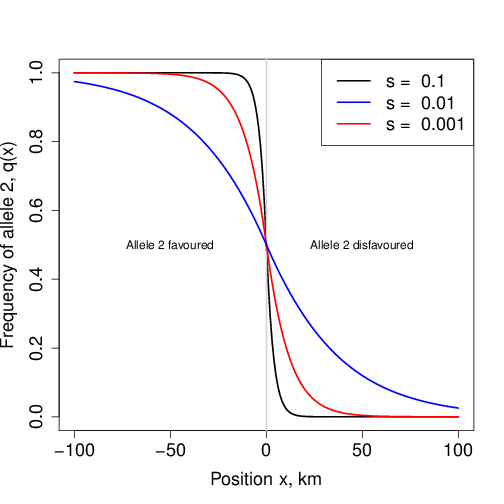
\includegraphics[width=0.5\textwidth]{figures/equilib_cline.png}
\end{center}
\caption{An equilibrium cline in allele frequency. Our individuals
  dispersal an average distance of $\sigma=1$km per generation, and our
allele $2$ has a relative fitness of $1+s$ and $1-s$ on either side of
the environmental change at $x=0$.} \label{fig:cline}
\end{figure}

\paragraph{The cline in allele frequency associated with a sharp
  environmental transition.}
To make progress lets consider a simple model of location adaptation where the
environment abruptly changes. Specifically we assume that $\gamma(x)= 1$ for
$x<0$ and $\gamma(x)= -1$ for $x \geq 0$, i.e. our allele $2$ has a selective
advantage at locations to the left of zero, while this allele is at a
disadvantage to the right of zero. In this case we can get an equilibrium
distribution of our two alleles were to the left of $zero$ our allele $2$ is at
higher frequency, while to the right of zero allele $1$ predominates. As we
cross from the left to the right side of our range the frequency of our allele
$2$ decreases in a smooth cline.\\



%Under such a model the change in frequency of allele $2$ at location $x$ at time $t$,
%$q(x,t)$, over time follows the differential equation
%\begin{equation}
%\frac{dq(x,t)}{dt} = s\gamma(x) q(x,t) \left( 1 - q(x,t) \right) + \frac{\sigma^2}{2} \frac{d^2q(x,t)}{dx^2}
%\end{equation}
%the first term on the right-hand side is the logistic growth of our
%favoured allele at location $x$, while the second term on the
%right-hand side is the diffusion of allele frequencies due to
%dispersal (i.e. dispersal is acting to spread out the effect of
%allele frequency change across populations). See below for how we
%derive this \gc{to be added}.\\

Our equilibrium spatial distribution of allele frequencies can be found by
setting the LHS of eqn. \eqref{eqn:fisherKPP} to zero to arrive at
\begin{equation}
s\gamma(x) q(x) \left( 1 - q(x) \right) = - \frac{\sigma^2}{2} \frac{d^2q(x)}{dx^2}
\end{equation}
We then could solve this differential equation with appropriate boundary
conditions ($q(-\infty)=1$ and $q(\infty) = 0$) to arrive at the
appropriate functional form to our cline. While we won't go into the
solution of this equation here, we can note that by dividing our
distance $x$ by $\ell=\sigma/\sqrt{s}$ we can remove the effect of our
parameters from the above equation. This compound parameter $\ell$ is the characteristic
length of our cline, and it is this parameter which determines over
what geographic scale we change from allele $2$ predominating to
allele $1$ predominating as we move across our environmental shift. \\

The width of our cline, i.e. over what distance do we make this shift
from allele $2$ predominating to allele $1$,
can be defined in a number of different ways. One simple way to define
the cline width, which is easy to define but perhaps hard to measure accurately, is the slope (i.e. the
tangent) of $q(x)$ at $x=0$. Under this definition the cline width is approximately $0.6
\sigma/\sqrt{s}$.\\

\paragraph{The rate of spatial spread of a beneficial allele.}
Consider a beneficial mutation that has arisen in a specific spatial
location and has begun to spread geographically. 
\gc{FINISH THIS.}


\newpage
